 
\chapter{Ordinary Least Squares (OLS) with a Univariate Covariate}
 \label{chapter::ols-1d}

\section{Univariate ordinary least squares}
Figure \ref{fig::galton_data_scatterplot} shows the scatterplot of Galton's dataset which can be found in the \ri{R} package \ri{HistData} as \ri{GaltonFamilies}. In this dataset, \ri{father} denotes the height of the father and \ri{mother} denotes the height of the mother. 
 The x-axis denotes the mid-parent height, calculated as (\ri{father} + 1.08*\ri{mother})/2, and the y-axis denotes the height of a child. 



\begin{figure}[ht]
\centering
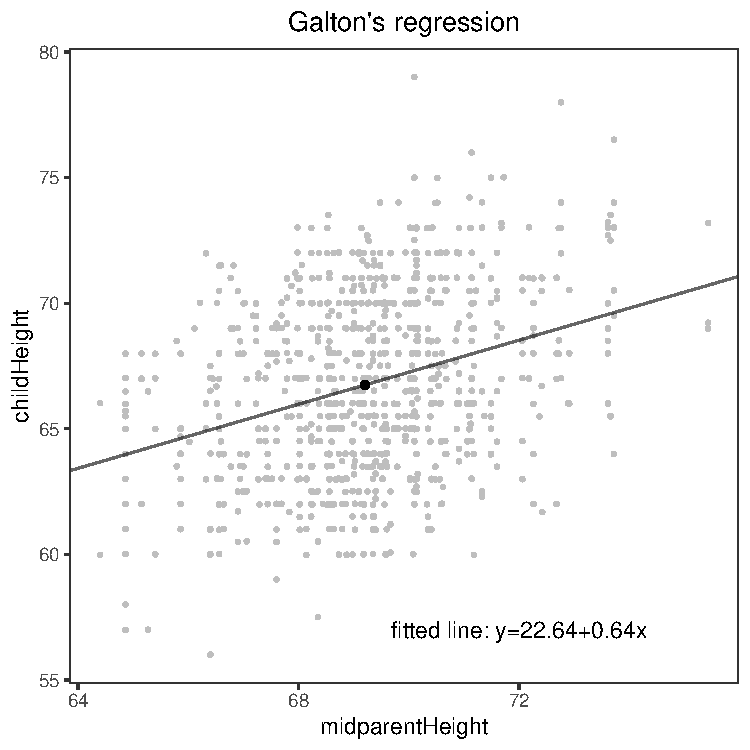
\includegraphics[width= 0.7\textwidth]{figures/galton_data_ggplot.pdf}
\caption{Galton's dataset}\label{fig::galton_data_scatterplot}
\end{figure}


With $n$ data points $(x_{i,}y_{i})_{i=1}^{n}$, our goal is to find the best linear fit of the data
\[
(x_{i,}\hat{y}_{i}=\hat{\alpha}+\hat{\beta}x_{i})_{i=1}^{n}.
\]
What do we mean by the ``best'' fit? Gauss proposed to use the following
criterion, called the ordinary least squares (OLS) \footnote{The idea of OLS is often attributed to Gauss and Legendre. Gauss used it in the process of discovering Ceres, and his work was published in 1809. Legendre's work appeared in 1805 but Gauss claimed that he had been using it since 1794 or 1795. \citet{stigler1981gauss} reviews the history of OLS.}:
\[
(\hat{\alpha},\hat{\beta})=\arg\min_{a,b}n^{-1}\sumn(y_{i}-a-b x_{i})^{2}.
\]

The OLS criterion is based on the squared ``misfits''
$y_{i}- a - b  x_{i}$. Another intuitive criterion is based
on the absolute values of those misfits, which is called the least
absolute deviation (LAD). However, OLS is simpler because the objective
function is smooth in $(a, b)$. We will discuss LAD in Chapter \ref{chapter::quantile-regression}. 


How to solve the OLS minimization problem? The objective function
is quadratic, and as $a$ and $b$ diverge, it diverges to
infinity. So it must has a unique minimizer $(\hat{\alpha},\hat{\beta})$
which satisfies the first-order condition:
\[
\begin{cases}
-\frac{2}{n}\sumn(y_{i}-\hat{\alpha}-\hat{\beta}x_{i}) & =0,\\
-\frac{2}{n}\sumn x_{i}(y_{i}-\hat{\alpha}-\hat{\beta}x_{i}) & =0.
\end{cases}
\]
These two equations are called the Normal Equations of OLS. The first
equation implies 
\begin{equation}
\bar{y}=\hat{\alpha}+\hat{\beta}\bar{x},\label{eq:normal1}
\end{equation}
that is, the OLS line must go through the sample mean of the data
$(\bar{x},\bar{y}).$ The second equation implies
\begin{equation}
\overline{xy}=\hat{\alpha}\bar{x}+\hat{\beta}\overline{x^{2},}\label{eq:normal2}
\end{equation}
where $\overline{xy}$ is the sample mean of the $x_{i}y_{i}$'s, and $\overline{x^{2}}$
is the sample mean of the $x_{i}^{2}$'s. Subtracting (\ref{eq:normal1})$\times\bar{x}$
from (\ref{eq:normal2}), we have
\begin{eqnarray*}
\overline{xy} - \bar{x} \bar{y} &=& \hat{\beta} ( \overline{x^{2}} - \bar{x}^2 ) \\
\Longrightarrow \hat{\sigma}_{xy} &=&\hat{\beta} \hat{\sigma}_{x}^2  \\
\Longrightarrow \hat{\beta}&=&  \frac{\hat{\sigma}_{xy}}{\hat{\sigma}_{x}^2}. 
\end{eqnarray*}
%where $\hat{\cov}$ and $\hat{\var}$ denote the sample covariance and variance. 
So the OLS coefficient of $x$ equals the sample covariance between
$x$ and $y$ divided by the sample variance of $x$. From (\ref{eq:normal1}),
we obtain that 
\[
\hat{\alpha}=\bar{y}-\hat{\beta}\bar{x}.
\]

Finally, the fitted line is
\begin{align*}
&y  =\hat{\alpha}+\hat{\beta}x=\bar{y}-\hat{\beta}\bar{x}+\hat{\beta}x\\
&\Longrightarrow y-\bar{y}=\hat{\beta}(x-\bar{x})\\
 & \Longrightarrow y-\bar{y}= \frac{   \hat{\sigma}_{xy}  }{  \hat{\sigma}_{x}^2  }(x-\bar{x})
 =\frac{  \hat{\rho}_{xy} \hat{\sigma}_{x}\hat{\sigma}_{y}}{\hat{\sigma}_{x}^{2}}(x-\bar{x})\\
 & \Longrightarrow\frac{y-\bar{y}}{\hat{\sigma}_{y}}= \hat{\rho}_{xy}  \frac{x-\bar{x}}{\hat{\sigma}_{x}},
\end{align*}
which is the Galtonian formula mentioned in Chapter \ref{chapter::motivation}. 

%Why statistics? The above OLS results are purely algebraic, that is,
%finding the best linear fit to $n$ points. If this is the only goal,
%then we do not need to impose any additional assumptions in the above
%procedure. However, we want to make inference based on OLS. Here inference
%means quantifying uncertainty. But before quantifying uncertainty,
%we need to explicitly state the truth we want to infer. 
%
%
%One possible
%model is that $(x_{i},y_{i})_{i=1}^{n}$ are IID and
%\[
%y_{i}=\alpha+\beta x_{i}+\varepsilon_{i}\qquad(i=1,\ldots,n)
%\]
%where the outcome variable $y_{i}$ on the left-hand side is generated
%based on $x_{i}$ and $\varepsilon_{i}$ on the right-hand side. We
%can view the $\varepsilon_{i}$ term as random errors that satisfies
%\[
%\begin{cases}
%E(\varepsilon_{i}) & =0,\\
%E(\varepsilon_{i}x_{i}) & =0.
%\end{cases}
%\]
%
%Under this model, $(x_{i},y_{i})_{i=1}^{n}$ are random, so are $\hat{\alpha}$
%and $\hat{\beta}$. Then we can discuss the distributional properties
%of $\hat{\alpha}$ and $\hat{\beta}$, for example, their means, variances,
%and sampling distributions. 
%\section{Galton's data}


We can obtain the fitted line based on Galton's data using the \ri{R} code below. 

\begin{rc}
> library("HistData")
> xx = GaltonFamilies$midparentHeight
> yy = GaltonFamilies$childHeight
> 
> center_x = mean(xx)
> center_y = mean(yy)
> sd_x     = sd(xx)
> sd_y     = sd(yy)
> rho_xy   = cor(xx, yy)
> 
> beta_fit  = rho_xy*sd_y/sd_x
> alpha_fit = center_y - beta_fit*center_x
> alpha_fit
[1] 22.63624
> beta_fit
[1] 0.6373609
\end{rc}

This generates Figure \ref{fig::galton_data_scatterplot}. 




\section{Final comments}

We can write the sample mean as the solution to the OLS with only the intercept:
$$
\bar{y} = \arg\min_{\mu}n^{-1}\sumn(y_{i} - \mu)^{2}.
$$


It is rare to fit OLS of $y_i$ on $x_i$ without the intercept: 
\[
 \hat{\beta}=\arg\min_{b}n^{-1}\sumn(y_{i} -b x_{i})^{2} 
\]
which equals 
$$
 \hat{\beta} 
 = \frac{ \sumn x_iy_i }{  \sumn x_i^2 } = \frac{  \langle x, y \rangle   }{ \langle x, x \rangle } , 
 $$
 where $x$ and $y$ are the $n$-dimensional vectors containing all observations, and $\langle x, y \rangle = \sumn x_iy_i$ denotes the inner product. 
Although not directly useful, this formula will be the building block for many discussions later. 


\section{Homework problems}

  

\paragraph{Pairwise slopes}\label{hw2::pairwise-slope}
Given $(x_i, y_i)_{i=1}^n$ with univariate $x_i$ and $y_i$, show that Galton's slope equals
$$
\hat{\beta} = \sum_{(i,j)} w_{ij} b_{ij},
$$
where the summation is over all pairs of observations $(i,j)$, 
$$
b_{ij} = (y_i - y_j ) / (x_i - x_j ) 
$$
is the slope determined by two points $(x_i,y_i)$ and $(x_j, y_j)$, and 
$$
w_{ij} = (x_i - x_j)^2 / \sum_{(i',j')} (x_{i'} - x_{j'})^2
$$
is the weight proportional to the squared distance between $x_i$ and $x_j$. In the above formulas, we define $b_{ij} = 0$ if $x_i=x_j$.

Remark: \citet{wu1986jackknife} and
\citet{gelman2009splitting} used this formula. 
Problem \ref{hw03::jacobi} gives a more general result. 


 
